\documentclass{standalone}
\usepackage{tikz}

\begin{document}
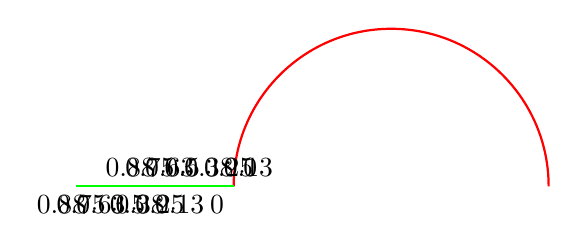
\begin{tikzpicture}[scale=2]
    % Draw the arc
    \draw[red, thick] (0,0) arc (180:0:1);
    
    % Draw the green lines
    \foreach \x in {0, 0.125, ..., 0.875} {
        \draw[green, thick] ({\x*cos(180)}, {\x*sin(180)}) -- ({(\x+0.125)*cos(180)}, {(\x+0.125)*sin(180)});
    }
    
    % Draw the labels
    \foreach \x in {0, 0.125, ..., 0.875} {
        \node at ({\x*cos(180)}, {\x*sin(180)}) [above right] {\pgfmathprintnumber{\x}};
    }
    
    % Draw the red labels
    \foreach \x in {0, 0.125, ..., 0.875} {
        \node at ({\x*cos(180)}, {\x*sin(180)}) [below left] {\pgfmathprintnumber{\x}};
    }
\end{tikzpicture}
\end{document}